\documentclass[%
    a0paper,%
    20pt,%
    portait,%
    margin=0mm,%
    innermargin=10mm,%
    blockverticalspace=10mm,%
    colspace=10mm,%
    subcolspace=5mm%
]{tikzposter}

%%% Local Variables:
%%% TeX-master: "poster"
%%% End:

% ==============================================================================
% Packages
% ==============================================================================
\usepackage[utf8]{inputenc}
\usepackage[T1]{fontenc}
\usepackage[        % use biblatex for bibliography
    backend=biber,  % use biber backend (bibtex replacement) or bibtex
    style=ieee,     % bib style
    natbib=true,    % allow natbib commands
    hyperref=true,  % activate hyperref support
    backref=false,  % activate backrefs
    isbn=false,     % don't show isbn tags
    url=false,      % don't show url tags
    doi=false,      % don't show doi tags
    urldate=long,   % display type for dates
    maxnames=3,     %
    minnames=1,     %
    maxbibnames=5,  %
    minbibnames=3,  %
    maxcitenames=2, %
    mincitenames=1  %
]{biblatex}

\usepackage[english]{babel}  % Last language is main language
\usepackage{lmodern}         % Latin Modern Font
\usepackage{amssymb}
\usepackage{gensymb}         % Generic symbols for both text and math mode
\usepackage{amsmath}         % Main math Package
\usepackage{mathtools}       % Extension package to amsmath
\usepackage{amsthm}          % Typesetting theorems (AMS style)
\usepackage{amsfonts}        % More fonts from the AMS
\usepackage{textcomp}        % provide many text symbols
\usepackage{xstring}         % Utils to manipulate strings
\usepackage{etoolbox}        % Add basic if/then and usefull functions
\usepackage{esvect}          % Beautyfull vectors
\usepackage{graphicx}        % Enhanced support for graphics
\usepackage{grffile}         % Used by matlab2tikz
\usepackage{microtype}       % typographic tuning
\usepackage{setspace}        % for line spacing, e.g. \onehalfspacing
\usepackage{csquotes}        % Nice display of quotations
\usepackage{blindtext}       % package for blind text
\usepackage{steinmetz}       % For phase symbol
\usepackage[load-configurations=abbreviations]{siunitx} % SI units
\usepackage{caption}
\usepackage{subcaption}
\usepackage{wrapfig}         % Wrap text around figure
\usepackage{tikz}
\usepackage{array}     % Basic table support
\usepackage{tabularx}  % Great for auto-sizing columns
\usepackage{booktabs}  % Professional-looking layout
\usepackage[most]{tcolorbox}
\usepackage[framemethod=TikZ]{mdframed}
\usepackage{enumitem}
\usepackage[table]{xcolor}%
\usepackage{authblk}

\usepackage[cache=false]{minted}
% ==============================================================================

\renewcommand\Affilfont{\itshape\large}

% ==============================================================================
% Remove credentials of tikzposter
\tikzposterlatexaffectionproofoff
% ==============================================================================


% ==============================================================================
% Change MakeTitle command
% ==============================================================================
\makeatletter
\newcommand\insertlogoright[2][]{\def\@insertlogoright{\includegraphics[#1]{#2}}}
\newcommand\insertlogoleft[2][]{\def\@insertlogoleft{\includegraphics[#1]{#2}}}
\newlength\LogoSep
\setlength\LogoSep{60pt}

\insertlogoright[height=6cm]{./img/logo_esrf.pdf}
\insertlogoleft[height=6cm]{./img/logo_pml.pdf}

\renewcommand\maketitle[1][]{  % #1 keys
    \normalsize
    \setkeys{title}{#1}
    % Title dummy to get title height
    \node[transparent,inner sep=\TP@titleinnersep, line width=\TP@titlelinewidth, anchor=north, minimum width=\TP@visibletextwidth-2\TP@titleinnersep]
        (TP@title) at ($(0, 0.5\textheight-\TP@titletotopverticalspace)$) {\parbox{\TP@titlewidth-2\TP@titleinnersep}{\TP@maketitle}};
    \draw let \p1 = ($(TP@title.north)-(TP@title.south)$) in node {
        \setlength{\TP@titleheight}{\y1}
        \setlength{\titleheight}{\y1}
        \global\TP@titleheight=\TP@titleheight
        \global\titleheight=\titleheight
    };

    % Compute title position
    \setlength{\titleposleft}{-0.5\titlewidth}
    \setlength{\titleposright}{\titleposleft+\titlewidth}
    \setlength{\titlepostop}{0.5\textheight-\TP@titletotopverticalspace}
    \setlength{\titleposbottom}{\titlepostop-\titleheight}

    % Title style (background)
    % \TP@titlestyle

    % Title node
    \node[inner sep=\TP@titleinnersep, line width=\TP@titlelinewidth, anchor=north, minimum width=\TP@visibletextwidth-2\TP@titleinnersep]
        at (0,0.5\textheight-\TP@titletotopverticalspace)
        (title)
        {\parbox{\TP@titlewidth-2\TP@titleinnersep}{\TP@maketitle}};

    \node[inner sep=0pt,anchor=west]
      at ([xshift=\LogoSep]title.west)
      {\@insertlogoleft};

    \node[inner sep=0pt,anchor=east]
      at ([xshift=-\LogoSep]title.east)
      {\@insertlogoright};

    % Settings for blocks
    \normalsize
    \setlength{\TP@blocktop}{\titleposbottom-\TP@titletoblockverticalspace}
}

\def\title#1{\gdef\@title{\scalebox{\TP@titletextscale}{%
      \begin{minipage}[t]{\linewidth}
        \centering
        #1
        \par
        \vspace{0.5em}
      \end{minipage}%
    }}}
\makeatother
% ==============================================================================


% ==============================================================================
% Create Table Environment
% ==============================================================================
\makeatletter
\newcounter{tablecounter}
\newenvironment{tikztable}[1][]{
  \def \rememberparameter{#1}
  \vspace{10pt}
  \refstepcounter{tablecounter}
  \begin{center}
  }{
    \ifx\rememberparameter\@empty
    \else
    \\[10pt]
    {\small Tab.~\thetablecounter: \rememberparameter}
    \fi
  \end{center}
}
\makeatother
% ==============================================================================


% ==============================================================================
% Change block style
% ==============================================================================
\defineblockstyle{customstyle}{
    titlewidthscale=1, bodywidthscale=1, titlecenter,
    titleoffsetx=0pt, titleoffsety=0pt, bodyoffsetx=0pt, bodyoffsety=0pt,
    bodyverticalshift=0pt, roundedcorners=2, linewidth=2mm,
    titleinnersep=5mm, bodyinnersep=1cm
}{
    \begin{scope}[line width=\blocklinewidth, rounded corners=\blockroundedcorners]
        \ifBlockHasTitle %
           \draw[color=blocktitlebgcolor, fill=blocktitlebgcolor] (blockbody.south west) rectangle (blocktitle.north east);
           \draw[color=blocktitlebgcolor, fill=blockbodybgcolor] (blockbody.south west) rectangle (blockbody.north east);
        \else
           \draw[color=blocktitlebgcolor, fill=blockbodybgcolor] (blockbody.south west) rectangle (blockbody.north east);
        \fi
    \end{scope}
}
\usetheme{Default}
\usebackgroundstyle{Empty}
% ==============================================================================


% ==============================================================================
% Simple TCMBOX environment
% ==============================================================================
\definecolor{maincolor}{HTML}{0066A7}

\newtcbox{\tcmbox}[1][blue]{colback=maincolor!5!white, colframe=maincolor,
  nobeforeafter,math upper,tcbox raise base, boxrule=1mm, boxsep=4mm}
\newtcolorbox{cbox}[3][]{colback=maincolor!5!white, colframe=maincolor, fonttitle=\bfseries, size=normal, toptitle=3mm, botttomtitle=3mm, boxrule=1mm, title=#1, #3}
% ==============================================================================


% ==============================================================================
\newlength{\seplinewidth}
\newlength{\seplinesep}
\setlength{\seplinewidth}{1mm}
\setlength{\seplinesep}{2mm}

\newcommand*{\sepline}{%
  \par
  \vspace{\dimexpr\seplinesep+.5\parskip}%
  \cleaders\vbox{%
    \begingroup % because of color
    \color{maincolor}%
    \hrule width\linewidth height\seplinewidth
    \endgroup
  }\vskip\seplinewidth
  \vspace{\dimexpr\seplinesep-.5\parskip}%
}
% ==============================================================================

% ==============================================================================
\definecolor{mycolor1}{RGB}{79,115,193}
\definecolor{mycolor2}{RGB}{213,91,53}
% ==============================================================================

% ==============================================================================
\AtBeginBibliography{\small}
% ==============================================================================

\addbibresource{ref.bib}

\author{Dehaeze Thomas, Verma Mohit and Collette Christophe}
\date{2019-11-06}
\title{Complementary Filters Shaping Using \scalebox{2}{$\mathcal{H}_\infty$} Synthesis}
\institute{}

\useblockstyle{customstyle}

\begin{document}

\maketitle[%
    roundedcorners=2,
    linewidth=2mm,
    innersep=10mm,
    titletotopverticalspace=10mm,
    titletoblockverticalspace=10mm]

\block[]{}{\textbf{Abstract}
For many applications, large bandwidth and dynamic ranges are requiring to use several sensors, whose signals are combined using complementary filters.
This paper presents a method for designing these complementary filters using $\mathcal{H}_\infty$ synthesis that allows to shape the filter norms.
This method is shown to be easily applicable for the synthesis of complex complementary filters.
}

\begin{columns}
\column{0.5}
\block[]{Introduction}{A set of filters is said to be complementary if the sum of their transfer functions is equal to one at all frequencies.
These filters are used when two or more sensors are measuring the same physical quantity with different noise characteristics. Unreliable frequencies of each sensor are filtered out by the complementary filters and then combined to form a super sensor giving a better estimate of the physical quantity over a wider bandwidth.
This technique is called sensor fusion and is used in many applications.\par

In \cite{zimmermann92_high_bandw_orien_measur_contr,corke04_inert_visual_sensin_system_small_auton_helic,min15_compl_filter_desig_angle_estim}, various sensors (accelerometers, gyroscopes, vision sensors, etc.) are merged using complementary filters for the attitude estimation of Unmanned Aerial Vehicles (UAV).
In \cite{collette15_sensor_fusion_method_high_perfor}, several sensor fusion configurations using different types of sensors are discussed in order to increase the control bandwidth of active vibration isolation systems.
Furthermore, sensor fusion is used in the isolation systems of the Laser Interferometer Gravitational-Wave Observator (LIGO) to merge inertial sensors with relative sensors
\cite{matichard15_seism_isolat_advan_ligo,hua04_polyp_fir_compl_filter_contr_system}. \par

As the super sensor noise characteristics largely depend on the complementary filter norms, their proper design is of primary importance for sensor fusion.
In \cite{corke04_inert_visual_sensin_system_small_auton_helic,jensen13_basic_uas,min15_compl_filter_desig_angle_estim}, first and second order analytical formulas of complementary filters have been presented.
Higher order complementary filters have been used in
\cite{shaw90_bandw_enhan_posit_measur_using_measur_accel,zimmermann92_high_bandw_orien_measur_contr,collette15_sensor_fusion_method_high_perfor}.
In \cite{jensen13_basic_uas}, the sensitivity and complementary sensitivity transfer functions of a feedback architecture have been proposed to be used as complementary filters. The design of such filters can then benefit from the classical control theory developments.
Linear Matrix Inequalities (LMIs) are used in \cite{pascoal99_navig_system_desig_using_time} for the synthesis of complementary filters satisfying some frequency-like performance.
Finally, a synthesis method of high order Finite Impulse Response (FIR) complementary filters using convex optimization has been developed in \cite{hua05_low_ligo,hua04_polyp_fir_compl_filter_contr_system}. \par

Although many design methods of complementary filters have been proposed in the literature, no simple method that allows to shape the norm of the complementary filters is available.

This paper presents a new design method of complementary filters based on $\mathcal{H}_\infty$ synthesis.
This design method permits to easily shape the norms of the generated filters.}
\block[]{Complementary Filters Requirements}{\begin{tikzfigure}[Sensor fusion architecture]
  \label{fig:fusion_super_sensor}
  \centering
  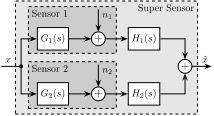
\includegraphics[scale=1.8]{figs/fusion_super_sensor.pdf}
\end{tikzfigure}

\begin{tikzfigure}[Sensor fusion architecture with sensor dynamics uncertainty]
  \label{fig:sensor_fusion_dynamic_uncertainty}
  \centering
  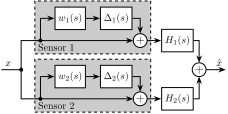
\includegraphics[scale=1.8]{figs/sensor_fusion_dynamic_uncertainty.pdf}
\end{tikzfigure}

\begin{tikzfigure}[Uncertainty set of the super sensor dynamics]
  \label{fig:uncertainty_set_super_sensor}
  \centering
  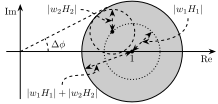
\includegraphics[scale=1.8]{figs/uncertainty_set_super_sensor.pdf}
\end{tikzfigure}}

\column{0.5}
\block[]{Complementary Filters Shaping using $\mathcal{H}_\infty$ Synthesis}{\begin{minipage}[t]{.6\linewidth}
  The \textbf{synthesis objective} is to \textbf{shape the norm of two filters}
  while ensuring their \textbf{complementary property}.
  This is equivalent to the conditions on the right where \(H_1(s)\) and
  \(H_2(s)\) are stable transfer function.
  $W_1(s)$ and $W_2(s)$ are \textbf{weighting functions} that are used to define
  wanted \textbf{upper bound of the complementary filter norms}.
  They should be \textbf{proper}, \textbf{stable} and \textbf{minimum phase}
  transfer functions.
\end{minipage}\hfill%
\begin{minipage}[t]{.38\linewidth}
  \vspace{-1em}
  \[ \tcmbox{\begin{align*}
       &H_1(s) + H_2(s) = 1 \\
       &|H_1(j\omega)| \le \frac{1}{|W_1(j\omega)|} \quad \forall\omega \\
       &|H_2(j\omega)| \le \frac{1}{|W_2(j\omega)|} \quad \forall\omega
     \end{align*}} \]
\end{minipage}

\bigskip

\begin{minipage}[t]{0.47\linewidth}
  This optimization problem is written as a \textbf{standard} \(\mathcal{H}_\infty\)
  \textbf{problem} (Fig.~\ref{fig:h_infinity_robust_fusion}).

  The \(\mathcal{H}_\infty\) synthesis applied to \(P(s)\) generates
  a stable filter \(H_2(s)\) such that the \(\mathcal{H}_\infty\) norm from \(w\) to \([z_1, \ z_2]\)
  is less than one.
  By defining \(H_1(s) \triangleq 1 - H_2(s)\), this is equivalent to the
  synthesis objective described above.
  \begin{tikzfigure}[$\mathcal{H}_\infty$ synthesis of
    complementary filters]
    \label{fig:h_infinity_robust_fusion}
    \centering
    \includegraphics[scale=1.8]{figs/h_infinity_robust_fusion.pdf}
  \end{tikzfigure}
\end{minipage}\hfill
\begin{minipage}[t]{0.49\linewidth}
  This \(\mathcal{H}_\infty\) synthesis is first applied for the design of simple complementary
  filters (Fig.~\ref{fig:hinf_synthesis_results}).

  \begin{tikzfigure}[Frequency response of the weighting functions and
    complementary filters obtained using $\mathcal{H}_\infty$ synthesis]
    \label{fig:hinf_synthesis_results}
    \centering
    \includegraphics[width=\linewidth]{figs/hinf_synthesis_results.pdf}
  \end{tikzfigure}
\end{minipage}

%%% Local Variables:
%%% TeX-master: "poster"
%%% End:}
\block[]{Application: Design of Complementary Filters used in the Active Vibration Isolation System at the LIGO}{%%% Local Variables:
%%% TeX-master: "poster"
%%% End:

The specifications for one pair of complementary filters used at the LIGO are
detailed in \cite{hua04_polyp_fir_compl_filter_contr_system} and shown in the
frequency domain in Fig.~\ref{fig:ligo_weights}.

\begin{minipage}[t]{0.49\linewidth}
  \begin{tikzfigure}[Specifications and weighting functions magnitude used for $\mathcal{H}_\infty$ synthesis]
    \label{fig:ligo_weights}
    \centering
    \includegraphics[width=\linewidth]{figs/ligo_weights.pdf}
  \end{tikzfigure}
\end{minipage}\hfill
\begin{minipage}[t]{0.49\linewidth}
  \begin{tikzfigure}[Comparison of the FIR filters (solid) designed in \cite{hua05_low_ligo} with the filters obtained with $\mathcal{H}_\infty$ synthesis (dashed)]
    \label{fig:comp_fir_ligo_hinf}
    \centering
    \includegraphics[width=\linewidth]{figs/comp_fir_ligo_hinf.pdf}
  \end{tikzfigure}
\end{minipage}
}
\block[]{Conclusion}{%%% Local Variables:
%%% TeX-master: "poster"
%%% End:

Complementary filters can be used to \textbf{combine multiple sensors} in order
to obtain a \textbf{super sensor}.
Specification on the super sensor \textbf{noise} and on the \textbf{robustness
  of the sensor fusion} are linked to the \textbf{norm of the complementary filters}.
A synthesis method that permits the \textbf{shaping of the complementary filters
  norms} has been proposed and has been successfully applied for the design of
complex filters.
\vspace{0.5em}
}
\end{columns}

\block[]{}{\textbf{Reference}
\printbibliography[heading=none]

\textbf{Acknowledgments}
This research benefited from a FRIA grant from the French Community of Belgium.
}

\end{document}